\spaltenanfang
Wir schreiben das Jahr 2050. Im Madison Cube Garden stehen sich 11 menschliche und 10 Roboter-Fußballer gegenüber. Moment, 10? Da fehlt doch einer! Aha, Bender steht rauchend und trinkend auf der VIP-Tribüne und klaut Schmuck und Uhren!
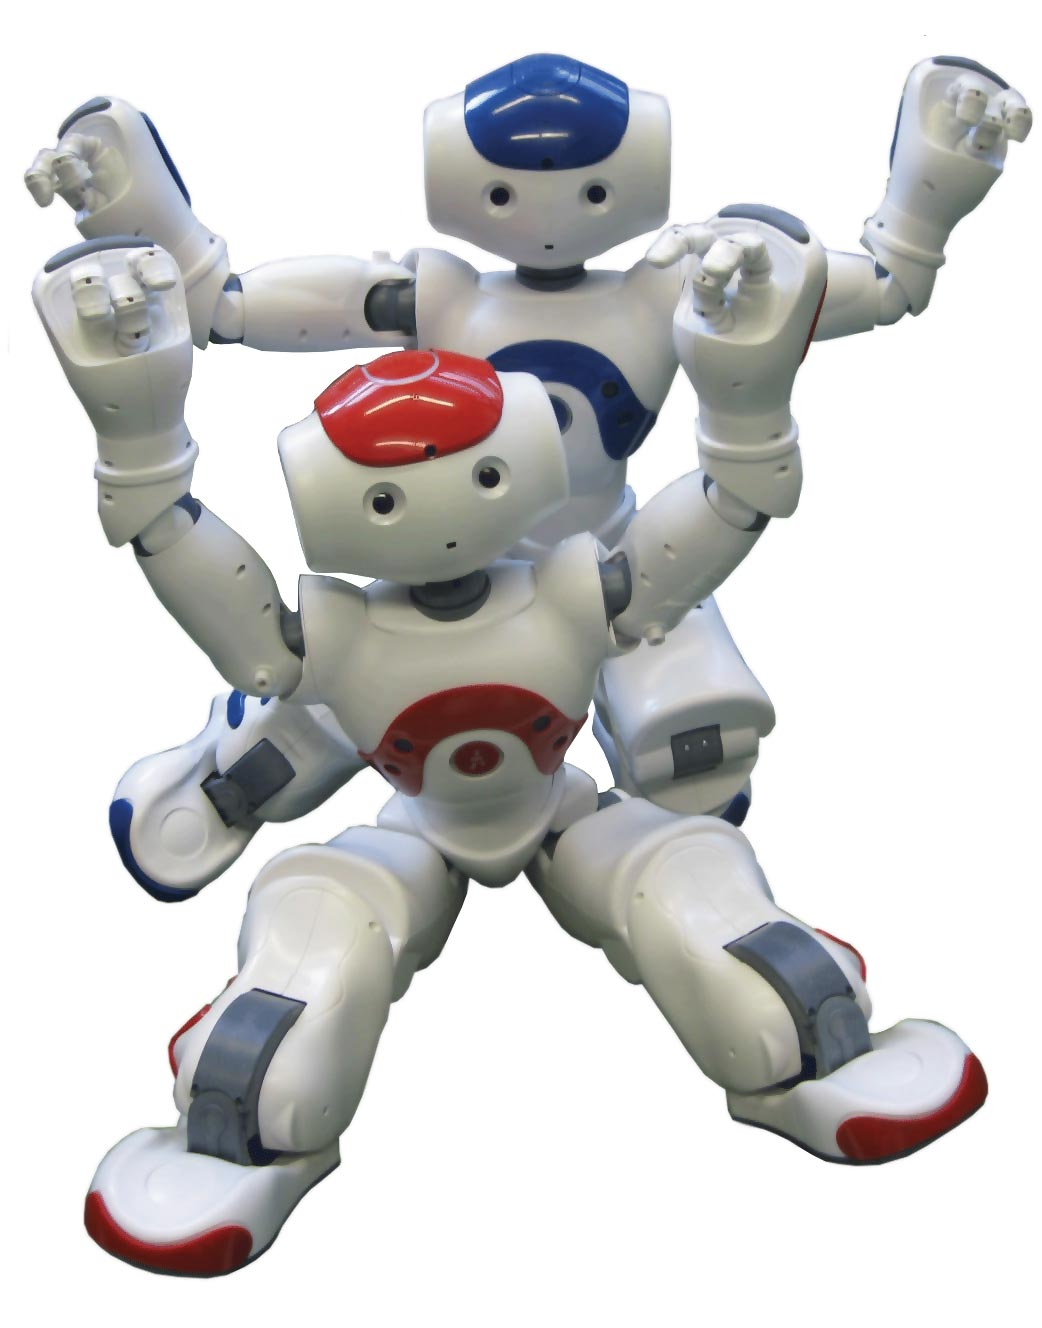
\includegraphics[width=8cm]{bilder/robocup1}

So oder ähnlich oder komplett anders könnte die Zukunft aussehen, wenn DU bei unserem Team mitmachst!

Doch blicken wir zurück ins Jahr 2009, wo alles seinen Anfang fand. Mittlerweile hat schon fast jede Erd-Universität eigene Prototypen, unter anderem auch die Robocup-AG der Universität Frankfurt. Die Vorform von Bender, Nao, hat noch bessere Manieren und sieht relativ harmlos aus, ist aber leider auch noch ziemlich unfähig. Und hier kommt das Team Bembelbots ins Spiel, die Studenten der Robocup-AG, die ihm Leben einhauchen. Unter der Schirmherrschaft des Joint Robotics Lab (JRL) arbeiten wir ständig an der Verbeserung von Nao's Fähigkeiten.

Unabhängig vom Kenntnisstand findet sich bei uns für jeden eine Aufgabe, der RoboCup bietet für jeden Teilbereich der Informatik spezielle Herausforderungen. So kann man sich entscheiden, ob man mithilfe der Bildverarbeitung, Bewegungsoptimierung, Künstlicher Intelligenz, oder aber auf einem ganz anderen Weg unserem Roboter zum Erfolg verhilft.

Und mit etwas Glück erfüllen wir das oben aufgeführte Szenario von Professor Farnsworths ``Was wäre, wenn?''-Maschine und lassen unsere Roboter wirklich irgedwann gegen menschliche Gegner antreten. Wenn du interessiert bist, mitmachen oder einfach mal reingucken willst, bist du herzlich eingeladen in der Robert-Mayer-Straße 11-15, Raum 19-20 vorbeizukommen, oder du besuchst unsere Internet-Seite zum Robocup/JRL:
 
\url{http://www.bembelbots.de}

Hier findest du neben Infos zum Robocup auch andere studentische Projekte des Joint Robotics Lab. 
\spaltenende

\includegraphics[width=0.8\textwidth]{bilder/Bembelbots}
